\chapter{Calculator With Friendly Output}
\label{chapter:calc}
\graphicspath{{./Lab06Calculator/Fig}}

\section{Outcomes and Objectives}

The outcome of this lab is to instantiate a calculator with signed
decimal output making it easy for anyone to use the circuit.
Through this process you will achieve the following
learning objectives.
\begin{itemize}
    \item \Paste{bok:CC_WireLogic}
    \item \Paste{bok:CC_Glue_Combo}
    \item \Paste{bok:CC_Combos}
    \item \Paste{VER:AlwaysCaseZ}
    \item\Paste{HDL:Synthesis}
\end{itemize}

\section{Calculator with Friendly Output}

This week you are going to build a calculator that can add or
subtract 4-bit values using the input and output shown in
Figure~\ref{fig:calcDevBoard} and display the results as
decimal, base-10, values, not as hexadecimal values.

\begin{figure}[ht]
    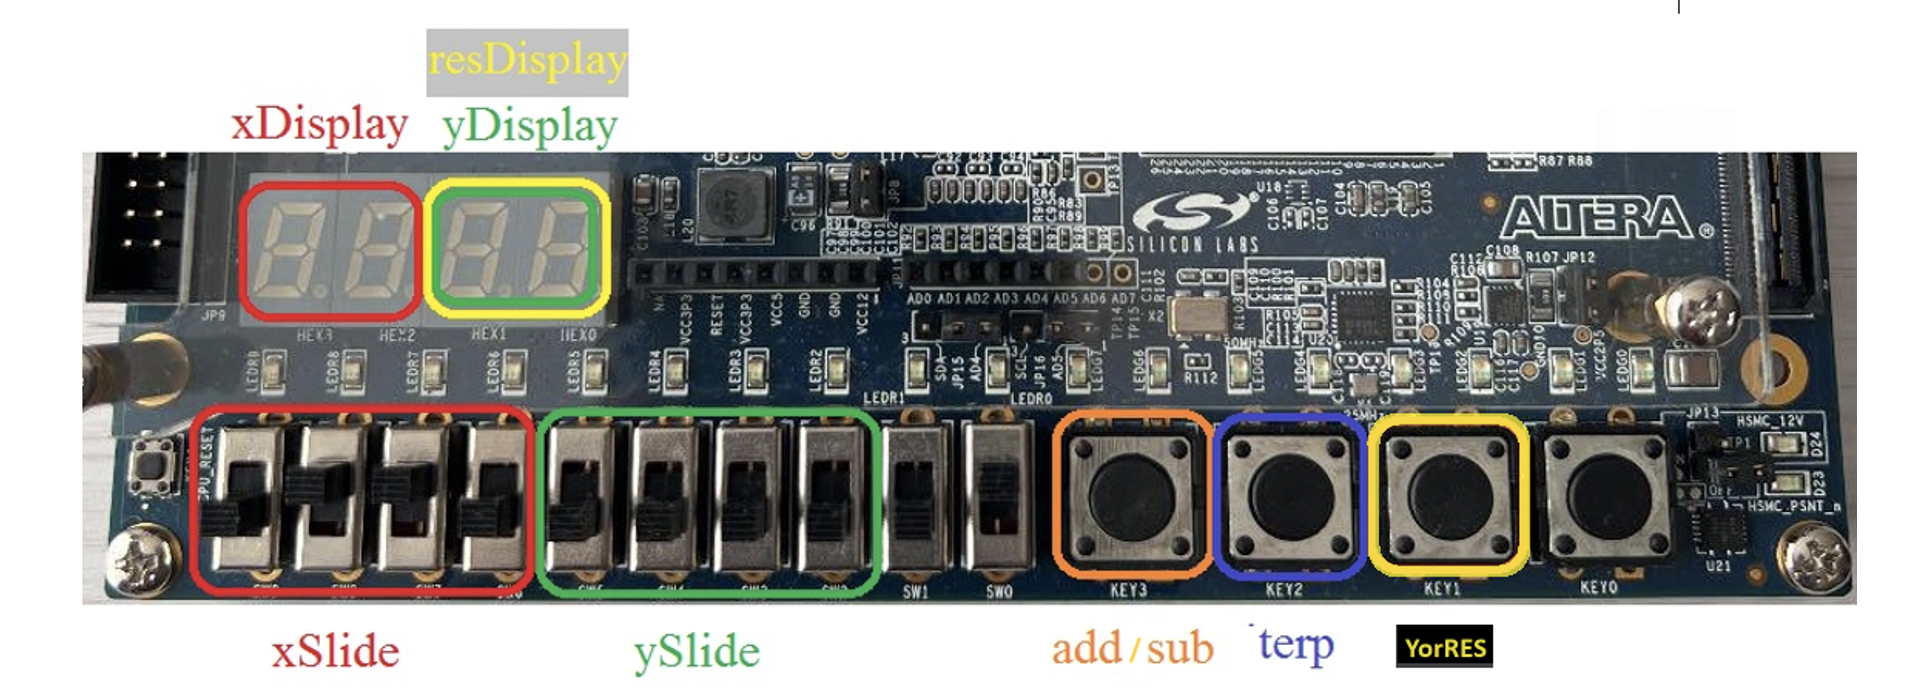
\includegraphics{ image1.png}
    \caption{The input and output of the calculator digital circuit.}
    \label{fig:calcDevBoard}
\end{figure}

On the surface, this should require nothing more
than connecting some slide switches to the x and y inputs of an
adder/subtractor which sends its output to a 7-segment display. And for
the most part this is correct. However, instead of displaying the input
and output of the adder as hexadecimal values, you will display them as
2-digit decimal values.

The user input and output are shown in Figure~\ref{fig:calcDevBoard}.
The user enters a pair of 4-bit operands using the left-most slide
switches, \device{xSlide} and \device{ySlide}. The value entered for
\device{xSlide} is displayed on the two (red) \device{xDisplay}
7-segment displays. The value entered for \device{ySlide} is displayed
on the two (green) \device{yDisplay} 7-segment displays. The leftmost
the \device{addSub} buttons specify the operation performed on
\device{xSlide} and \device{ySlide}. The result is \device{xSlide} +
\device{ySlide} or \device{xSlide} - \device{ySlide}.

The \device{interp} button determines how the values are displayed on the
7-segment display. When unpressed, the 7-segment displays show the
decimal value, when pressed, the 7-segment displays show 2's complement.
This will be explained in the next section. As we have only four 7-segment displays on
board, the same 7-segment displays of operand Y will be used to show the operation
result (yellow) when the \device{yOrResult} button is pressed.

\section{System Architecture}

The system architecture shown in Figure~\ref{fig:sysArchCalc} shows the adder subtractor
processing the \device{xSlide} and \device{ySlide} inputs. The 4-bit x, y and result
values are processed by the \hdl{sigUnsig} module before being displayed on the
7-segment displays. It is now time to turn our attention to this module.

\begin{figure}[ht]
    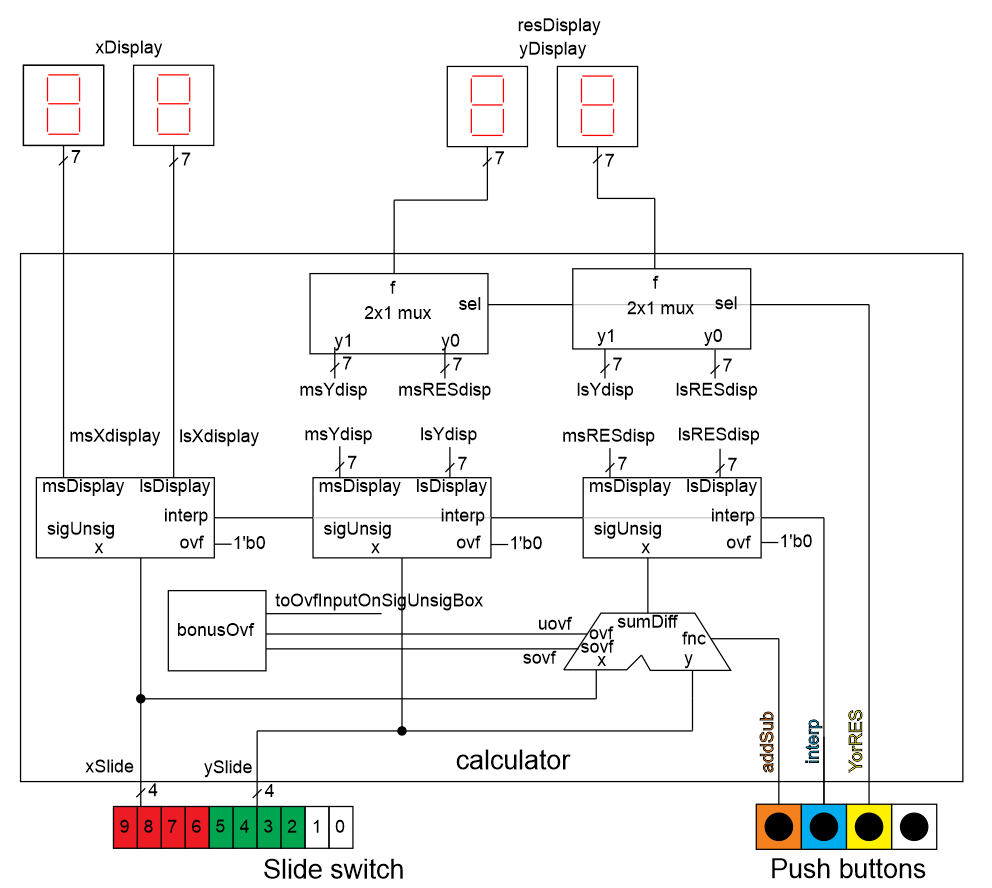
\includegraphics[width=0.5\paperwidth]{ image2.png}
    \caption{The system architecture of the calculator.}
    \label{fig:sysArchCalc}
\end{figure}

\section{Module: sigUnsign}

The significant design problem in today's lab comes in this section,
building the \hdl{sigUnsign} module that shows up three times in Figure~\ref{fig:sysArchCalc}.
This module takes in a 4-bit value and
displays a 2-digit signed or unsigned representation on a pair of
7-segment displays. The \hdl{sigUnsign} module declaration is shown in Listing~\ref{listing:cacSigUnsigModule}.

\begin{lstlisting}[language=Verilog,
 caption={Module declaration for the sigUnsig module.},
 label={listing:cacSigUnsigModule},
 frame=single]
 module sigUnsig(x, interp, ovf, msDisplay, lsDisplay);
    input  wire [3:0]  x;
    input  wire        interp;
    input  wire        ovf;
    output wire [6:0]  msDisplay, lsDisplay;
 \end{lstlisting}

The 4-bit input \hdl{x} is interpreted as either signed (2's complement
value) when \hdl{interp = 1} or unsigned (regular binary number) when
\hdl{interp = 0}.  The \device{msDisplay} is the most significant (ms)
symbol being displayed and \device{lsDisplay} is the least significant (ls)
symbol being display.  The term ``symbol'' is used because more than
one type of information can be displayed depending on the values
of the inputs.  Let's explore this.

For example, let \hdl{x = 4'b1100}.
\begin{itemize}
    \item
        If \hdl{interp = 1'b0} then
        \hdl{x} is interpreted as unsigned and its value is 12. Then
        the \device{msDisplay} should show ``1'' and \device{lsDisplay} ``2''.

    \item
        If \hdl{interp = 1'b1} then
        \hdl{x} is interpreted as 2's complement and its value is -4. Then
        the \device{msDisplay} should show ``-'' and \device{lsDisplay} ``4''.

    \item
        In the previous two cases we assumed, without stating it, that \hdl{ovf = 1'b0}.
        If \hdl{ovf = 1'b1} then the operation which generated \hdl{x} overflowed
        and the value of \hdl{x} is invalid.  In this case both display's should show ``X''.
        Since we are working with 7-segments, our ``X'' looks much more like ``H'' :(
    \end{itemize}

    Not complete Table~\ref{table:calcSigUnsign} by filling in the values of \hdl{msDisplay} and
    \hdl{lsDisplay} for a signed and unsigned interpretation, assuming
    \emph{ovf}=0. If the interpreted value is
    positive and a single digit then assign \emph{msDisplay} blank. If the
    interpreted value is negative then assign \emph{msDisplay} ``-``. If the
    interpreted value is greater than 10, assign \emph{msDisplay} ``1''.

    \begin{longtable}[]{@{}
            |  >{\raggedright\arraybackslash}p{(\columnwidth - 8\tabcolsep) * \real{0.1999}}|
            >{\raggedright\arraybackslash}p{(\columnwidth - 8\tabcolsep) * \real{0.2000}}|
            >{\raggedright\arraybackslash}p{(\columnwidth - 8\tabcolsep) * \real{0.2000}}|
            >{\raggedright\arraybackslash}p{(\columnwidth - 8\tabcolsep) * \real{0.2000}}|
        >{\raggedright\arraybackslash}p{(\columnwidth - 8\tabcolsep) * \real{0.2000}}|@{}}
        \caption{The output of the \hdl{sigUnsig} module when \hdl{ovf=0}.}\label{table:calcSigUnsign}\tabularnewline
        \toprule()
        \multirow{2}{*}{4-bit input x} &
        \multicolumn{2}{>{\raggedright\arraybackslash}p{(\columnwidth - 8\tabcolsep) * \real{0.4000} + 2\tabcolsep}}{%
        \hdl{interp = 0} Unsigned }
        &
        \multicolumn{2}{|>{\raggedright\arraybackslash}p{(\columnwidth - 8\tabcolsep) * \real{0.4000} +
        2\tabcolsep}|@{}}{%
        \hdl{interp = 1} Signed } \\ \cline{2-5}

        &\hdl{msDisplay} & \hdl{lsDisplay} & \hdl{msDisplay} & \hdl{lsDisplay} \\

        \midrule()
        \endfirsthead
        \toprule()
        \multirow{2}{*}{4-bit input x} &
        \multicolumn{2}{>{\raggedright\arraybackslash}p{(\columnwidth - 8\tabcolsep) * \real{0.4000} + 2\tabcolsep}}{%
        \hdl{interp = 0} Unsigned }
        &
        \multicolumn{2}{|>{\raggedright\arraybackslash}p{(\columnwidth - 8\tabcolsep) * \real{0.4000} +
        2\tabcolsep}|@{}}{%
        \hdl{interp = 1} Signed } \\  \cline{2-5}

        &\hdl{msDisplay} & \hdl{lsDisplay} & \hdl{msDisplay} & \hdl{lsDisplay} \\
        \midrule()
        \endhead
        4'b0000 & blank & 0 & blank & 0 \\ \hline
        4'b0001 & & & & \\ \hline
        4'b0010 & & & & \\ \hline
        4'b0011 & & & & \\ \hline
        4'b0100 & & & & \\ \hline
        4'b0101 & & & & \\ \hline
        4'b0110 & & & & \\ \hline
        4'b0111 & & & & \\ \hline
        4'b1000 & & & & \\ \hline
        4'b1001 & & & & \\ \hline
        4'b1010 & & & & \\ \hline
        4'b1011 & & & & \\ \hline
        4'b1100 & 1 & 2 & - & 4 \\ \hline
        4'b1101 & & & & \\ \hline
        4'b1110 & & & & \\ \hline
        4'b1111 & & & & \\
        \bottomrule()
    \end{longtable}

    Take a moment and look at the patterns in Table~\ref{table:calcSigUnsign}.  You should make the
    following important observations.
    \begin{itemize}

        \item \hdl{msDisplay} is assigned one of four values
            \begin{itemize}
                \item  \hdl{blank} when the interpretation of \hdl{x} is an unsigned or signed value less than  10.
                \item \hdl{1} when the interpretation of \hdl{x} is an unsigned value greater than 10.
                \item \hdl{-} when the interpretation of \hdl{x} is a \textbf{signed value less than 0}.
                \item \hdl{X} (the invalid character)when the \hdl{ovf = 1}.
            \end{itemize}

        \item \hdl{lsDisplay} is assigned one of four values,
            \begin{itemize}
                \item \hdl{x} (the value of the \hdl{x} input) when the interpretation of \hdl{x} is a
                    unsigned or signed value less than 10.
                \item \hdl{x-10} when the interpretation of \hdl{x} is an unsigned value greater than 10.
                \item \hdl{0-x} when the interpretation of \hdl{x} is a \textbf{signed value less than 0}.
                \item \hdl{X} (the invalid character) when the \hdl{ovf = 1}.
            \end{itemize}
    \end{itemize}

    \subsubsection{Why are we taking the 2's complement of \hdl{x}?}

    Please take a moment and reflect on pair of rows where you are asked to interpret \hdl{x} as a
    \textbf{signed value less than 0}.
    Under a signed (2's complement) interpretation, if the most significant bit of \hdl{x} is 1 then the
    value of \hdl{x} is less than 0.
    In this case the \device{msDisplay}  7-segment display should be illuminated with a ``-'' to indicate
    negative.  The \device{lsDisplay} needs
    to show the negation of \hdl{x} because the negation of a negative number is a positive number and we can
    use a \hdl{hexToSevenSeg}
    module to display positive numbers.  This is a complex but important observation.

    If you follow the above reasoning, there is a need to form the 2's complement of \hdl{x} in certain input
    situations.  You will form the
    negation of \hdl{x} by subtracting \hdl{x} from 0, that is compute \hdl{0-x}.  You will do this by
    putting \hdl{4'b0000} on the \hdl{x} input
    of an \hdl{addSub}, put the sigUnsign input \hdl{x} on the \hdl{y} input of an \hdl{addSub}, and hardwire
    the \hdl{fnc} input to \hdl{1'b1} so that the
    \hdl{addSub} is hardwired to always subtract.

    Formalized the observations in a more algorithmic syntax by completing Listing~\ref{listing:calcDisplayLogic}.
    Do this by filling the values of \hdl{msDisplay} and \hdl{lsDisplay} for the different input conditions.  The
    values for these two signals are given in the two lists above.  Note that this code is NOT to be used in your
    actual code for this lab.

    \pagebreak

\begin{lstlisting}[language=Verilog,
 caption={Logic that determines the output of the 4:1 muxes in Figure~\ref{fig:calcSigUnSigArch}.},
 label={listing:calcDisplayLogic},
 frame=single]
if        ( (interp == 0) && (x < 10) ) {    // y0 input
    msDisplay =         lsDisplay =

} else if ( (interp == 0) && (x >= 10) ) {    // y1 input
    msDisplay =        lsDisplay =

} else if ( (interp == 1) && (x >= 0) ) {    // y0 input
    msDisplay =        lsDisplay =

} else if ( (interp == 1) && (x < 0) ) {    // y2 input
    msDisplay =         lsDisplay =

}
\end{lstlisting}

    Now that you know what should be displayed on  \device{msDisplay}
    and \device{lsDisplay}, let's look at how we an form these symbols on the
    7-segment displays.  In order to do this, you need Figure~\ref{fig:calcSevenSeg},
    the bit-order of the segments controlling the illumination o the segments. Remember
    that the segments are active low, meaning a logic 0 illuminates a
    segment. Thus, the 7-bit code 7'b0100100 illuminates the pattern ``2''.

    \begin{figure}[ht]
        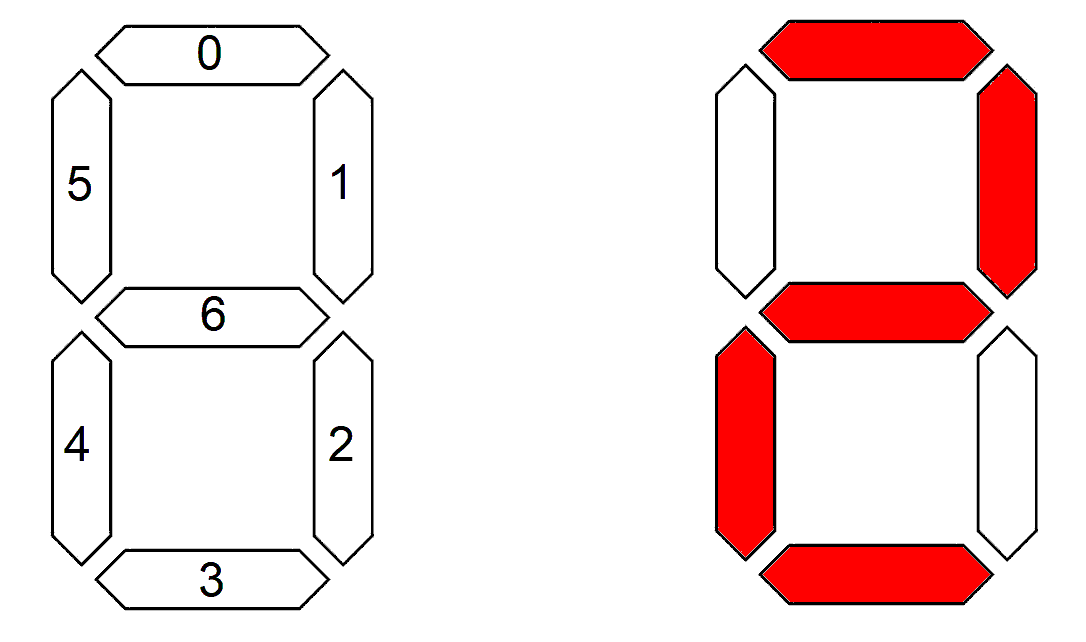
\includegraphics[width=0.3\paperwidth]{ image3.png}
        \caption{The logical arrangements of the segments in a 7-segment display.}
        \label{fig:calcSevenSeg}
    \end{figure}

    Test your understanding o the \hdl{signUnsign} output by completing
    Table~\ref{table:calcSevenSeg}. Do this by coloring in the segments of the
    7-segment displays that are illuminated for each of the inputs. Then write
    the binary and hexadecimal value to illuminate those patterns to the
    right of \hdl{msDisplay=7'b} and \hdl{lsDisplay=7'b}.

    \pagebreak

    \begin{longtable}[]{@{}
            |  >{\raggedright\arraybackslash}p{(\columnwidth - 8\tabcolsep) * \real{0.1458}}|
            >{\raggedright\arraybackslash}p{(\columnwidth - 8\tabcolsep) * \real{0.3170}}|
            >{\raggedright\arraybackslash}p{(\columnwidth - 8\tabcolsep) * \real{0.02}}|
            >{\raggedright\arraybackslash}p{(\columnwidth - 8\tabcolsep) * \real{0.1458}}|
        >{\raggedright\arraybackslash}p{(\columnwidth - 8\tabcolsep) * \real{0.3170}}|@{}}
        \caption{For each set of inputs to the signUnsig module, determine the 7-segment display
        pattern.}\label{table:calcSevenSeg} \tabularnewline
        \toprule()
        Input & 7-segment pattern & & Input & 7-segment pattern \\
        \midrule()
        \endfirsthead
        \toprule()
        Input & 7-segment pattern & & Input & 7-segment pattern \\
        \midrule()
        \endhead
        4'b0010

        interp = 1

        ovf = 0 &

        \vspace{0.1cm}
        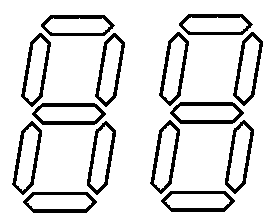
\includegraphics{ image4.png}
        \vspace{0.1cm}

        msDisplay = 7'b

        lsDisplay = 7'b & & 4'b0111

        interp = 0

        ovf = 0 &

        \vspace{0.1cm}
        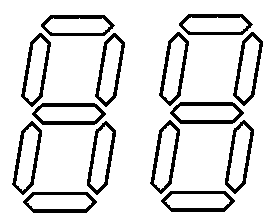
\includegraphics{ image4.png}
        \vspace{0.1cm}

        msDisplay = 7'b

        lsDisplay =7'b \\ \hline
        4'b1100

        interp = 0

        ovf = 0 &

        \vspace{0.1cm}
        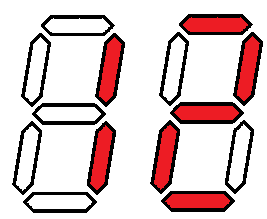
\includegraphics{ image5.png}
        \vspace{0.1cm}

        msDisplay = 7'b1111001 = 7'h79

        lsDisplay =7'b0100100 = 7'h24 & & 4'b1000

        interp = 1

        ovf = 0 &

        \vspace{0.1cm}
        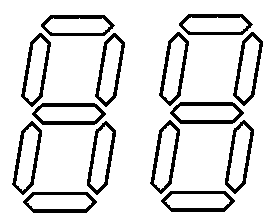
\includegraphics{ image4.png}
        \vspace{0.1cm}

        msDisplay = 7'b

        lsDisplay =7'b \\ \hline
        4'b1100

        interp = 1

        ovf = 0 &

        \vspace{0.1cm}
        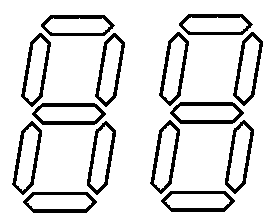
\includegraphics{ image4.png}
        \vspace{0.1cm}

        msDisplay = 7'b

        lsDisplay =7'b & & 4'b1010

        interp = 1

        ovf = 1 &

        \vspace{0.1cm}
        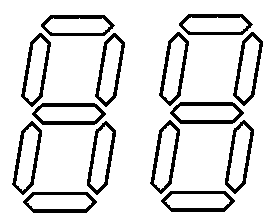
\includegraphics{ image4.png}
        \vspace{0.1cm}

        msDisplay = 7'b

        lsDisplay = 7'b \\ \hline
        \bottomrule()
    \end{longtable}

    Now we are ready to put the pieces of the sigUnsig module together. The
    building blocks in Figure~\ref{fig:calcSigUnSigArch} are captured in the organization described
    by Listing~\ref{listing:calcDisplayLogic}, along with some extra hardware.

    \begin{figure}[ht]
        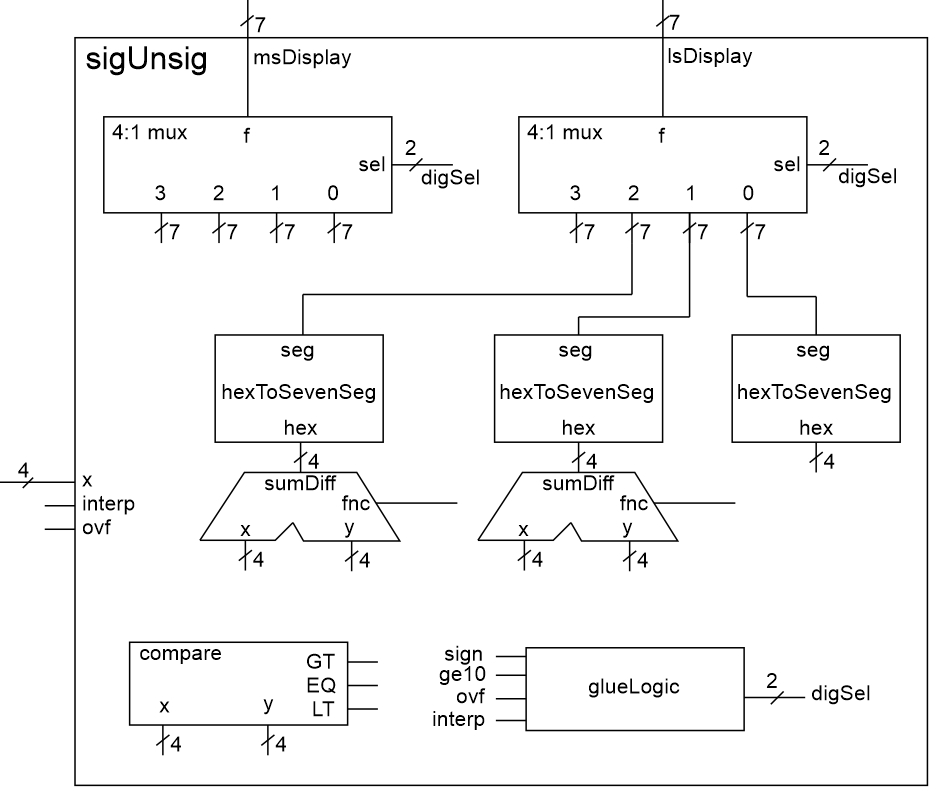
\includegraphics[width=0.5\paperwidth]{ image6.png}
        \caption{The internal architecture of the signUnsig module.}
        \label{fig:calcSigUnSigArch}
    \end{figure}

    Complete Figure~\ref{fig:calcSigUnSigArch} by adding the following:

    \begin{itemize}
        \item
            Connect the inputs of the 4:1 mux  using the logic described in Listing~\ref{listing:calcDisplayLogic}.
        \item
            Connect the inputs of the and adder subtractors using the logic described in
            Listing~\ref{listing:calcDisplayLogic}.
        \item
            Wire the inputs of the comparator to generate the signal \hdl{xGE10} which is
            logic 1 when \hdl{x} is greater than or equal to 10.
        \item
            Wire the input of the rightmost hexToSevenSeg .
    \end{itemize}

    Al that remains is to define the contents of the \hdl{glueLogic} box in Figure~\ref{fig:calcSigUnSigArch}.

    \subsubsection{\hdl{glueLogic} always/casez statement}

    the \hdl{glueLogic} box chooses which input of the 4 mux inputs to
    route to the output. This is the logic that you formalized in
    Listing~\ref{listing:calcDisplayLogic}.  Note the signal \hdl{sign} which equals 1 when \hdl{x}
    represents a negative value when interpreted as a signed value.

    Now complete the truth table in Table~\ref{table:calcGlueLogic} for the \hdl{glueLogic} box
    in Figure~\ref{fig:calcSigUnSigArch}.

    \begin{longtable}[]{@{}
            |  >{\raggedright\arraybackslash}p{(\columnwidth - 8\tabcolsep) * \real{0.1999}}|
            >{\raggedright\arraybackslash}p{(\columnwidth - 8\tabcolsep) * \real{0.2000}}|
            >{\raggedright\arraybackslash}p{(\columnwidth - 8\tabcolsep) * \real{0.2000}}|
            >{\raggedright\arraybackslash}p{(\columnwidth - 8\tabcolsep) * \real{0.2000}}|
        >{\raggedright\arraybackslash}p{(\columnwidth - 8\tabcolsep) * \real{0.2000}}|@{}}
        \caption{Truth table for the glueLogic box.}\label{table:calcGlueLogic}\tabularnewline
        \toprule()
        \begin{minipage}[b]{\linewidth}\raggedright
            \hdl{ovf}
        \end{minipage} &
        \begin{minipage}[b]{\linewidth}\raggedright
            \hdl{interp}
        \end{minipage} &
        \begin{minipage}[b]{\linewidth}\raggedright
            \hdl{sign}
        \end{minipage} &
        \begin{minipage}[b]{\linewidth}\raggedright
            \hdl{xGE10}
        \end{minipage} &
        \begin{minipage}[b]{\linewidth}\raggedright
            \hdl{digSel}
        \end{minipage} \\
        \midrule()
        \endfirsthead
        \toprule()
        \begin{minipage}[b]{\linewidth}\raggedright
            \hdl{ovf}
        \end{minipage} &
        \begin{minipage}[b]{\linewidth}\raggedright
            \hdl{interp}
        \end{minipage} &
        \begin{minipage}[b]{\linewidth}\raggedright
            \hdl{sign}
        \end{minipage} &
        \begin{minipage}[b]{\linewidth}\raggedright
            \hdl{xGE10}
        \end{minipage} &
        \begin{minipage}[b]{\linewidth}\raggedright
            \hdl{digSel}
        \end{minipage} \\
        \midrule()
        \endhead
        1 & x & x & x & \\ \hline
        0 & 0 & x & 0 & \\ \hline
        0 & 0 & x & 1 & \\ \hline
        0 & 1 & 0 & x & \\ \hline
        0 & 1 & 1 & x & \\
        \bottomrule()
    \end{longtable}

    It would make sense to use an always case statement to realize the logic
    in Listing~\ref{listing:calcDisplayLogic}. However, an always case statement requires each of the 16
    difference cases to be explicitly enumerated. However, the truth table
    in Listing~\ref{listing:calcDisplayLogic} is most efficiently described using don't cares in the
    input. Fortunately, the always/casez variation (note the ``z'' at the
    end of ``case'') allows don't cares in the input in the form of ``?''.
    For example, for the second row in Listing~\ref{listing:calcDisplayLogic}, the \{ovf, interp, sign,
    xGE10\} vector has don't cares for the \emph{sign} value. Therefore, the
    case for this row is 4'b01?0. \uline{It is imperative that you include a
    ``default'' case whenever you use a always/case statement.} This
    combination of cases is shown in Listing~\ref{listing:cacAlwaysStaement}.

\begin{lstlisting}[language=Verilog,
 caption={The always/casez statement allows don't cares in the input.},
 label={listing:cacAlwaysStaement},
 frame=single]
 always @(*)
    casez ({ovf, interp, xGE10, x[3]})
        4'b01?0: digSel = 2'b00;
        default: digSel = 2'b11;
    endcase

 \end{lstlisting}

    \subsubsection{\hdl{sigUnsig} Verilog code}
    \protect\hypertarget{sigUnsign_Verilog}{}{}
    The Verilog code for the
    signUnsig module consists of 8 instantiation statements and an
    always/casez statement. For this module, I want you to:

    \begin{itemize}
        \item
            Use the module declaration given in Listing~\ref{listing:cacSigUnsigModule}.
        \item
            Use the module definitions for

            \begin{itemize}
                \item
                    \hdl{genericMux4x1} posted on this lab's Canvas folder
                \item
                    \hdl{sevenSegment} created in lab 02
                \item
                    \hdl{genericAdderSubtractor} posted on a previous lab's Canvas folder
                \item
                    \hdl{genericComparator} posted on a previous lab's Canvas folder
            \end{itemize}
        \item
            Use localparm to give names to the 7-bit constant patterns (fill in
            the values for x).

            \begin{itemize}
                \item
                    \hdl{ localparam {[}6:0{]} displayBlank = 7'bxxxxxxx;}
                \item
                    \hdl{ localparam {[}6:0{]} displayOne = 7'bxxxxxxx;}
                \item
                    \hdl{ localparam {[}6:0{]} displayMinus = 7'bxxxxxxx;}
                \item
                    \hdl{ localparam {[}6:0{]} displayX = 7'bxxxxxxx;}
            \end{itemize}
        \item
            Provide meaningful names to the wires in the module.
        \item
            Properly tab-indent your code

            \begin{itemize}
                \item
                    Single level for wire declarations
                \item
                    Single level for component instantiations
                \item
                    Two levels for casez statement
                \item
                    Three levels for casez values
            \end{itemize}
    \end{itemize}

    \section{Testbench}
    \label{section:calcTestbench}
    Run the testbench for the sigUnsig module provided on Canvas. Produce
    a timing diagram with the following characteristics. Zoom to fill the
    available horizontal space with the waveform. Color inputs green and
    outputs red. Order the traces from top to bottom as

    \begin{tabular}{p{3cm}p{3cm}p{3cm}}
        signal            & radix                & Color for trace \\ \hline
        x radix         &    unsigned         & Green  \\
        xMinus10         &     unsigned     & Green  \\
        x                 &  decimal         & Cyan  \\
        negativeX         &  decimal         & Cyan  \\
        interp             & default             & Green  \\
        ovf             & default             & Green  \\
        digSel             &  unsigned         & Yellow  \\
        xGE10         & default             & Yellow  \\
        msDisplay         &  hex             & Red  \\
        lsDisplay         &  hex             & Red  \\
    \end{tabular}

    I do not want the signals from the testbench, but rather the signals
    from inside the \hdl{sigUnsig} module. You can do this in \hdl{sigUnsig} by
    expanding the \hdl{sigUnsig\_tb} instance in the left ModelSim pane and
    selecting ``uut''. Since uut is an instance of the \hdl{sigUnsig} module, all
    the signals accessible in the \hdl{sigUnsig} module are shown in the center
    Object. You can add duplicates of signals by repeating the drag-and-drop
    operation.

    Your completed timing diagram should look something like the following.

    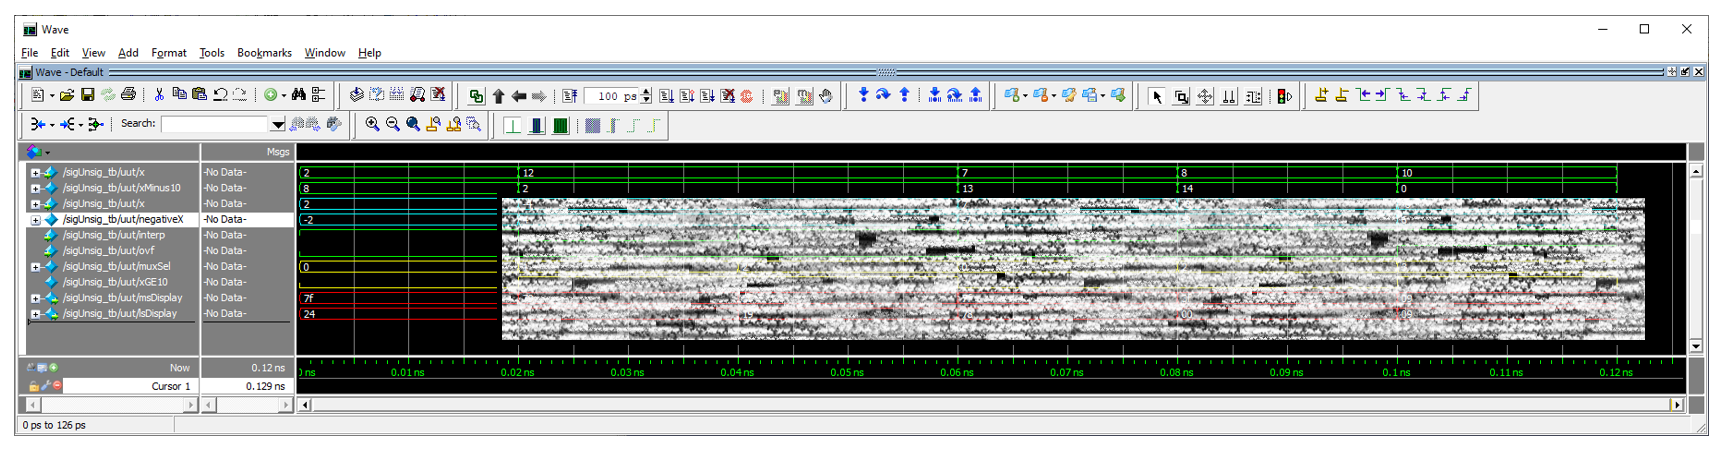
\includegraphics{ image7.png}

    \section{Pin-Assignment and Synthesis}

    Use the image of the FPGA Development Board in Figure~\ref{fig:calcDevBoard}
    and the information in the C5G User Guide to determine the FPGA pins associated
    with the input and output devices used by the devices used by the \hdl{calculator}
    module.

    \begin{longtable}[]{@{}
            |  >{\raggedright\arraybackslash}p{(\columnwidth - 8\tabcolsep) * \real{0.1436}}|
            >{\raggedright\arraybackslash}p{(\columnwidth - 8\tabcolsep) * \real{0.1829}}|
            >{\raggedright\arraybackslash}p{(\columnwidth - 8\tabcolsep) * \real{0.1665}}|
            >{\raggedright\arraybackslash}p{(\columnwidth - 8\tabcolsep) * \real{0.2621}}|
        >{\raggedright\arraybackslash}p{(\columnwidth - 8\tabcolsep) * \real{0.2448}}|@{}}
        \caption{Pin Assignment for the calculator.}\label{table:calcPinAssignment}\tabularnewline
        \toprule()
        \begin{minipage}[b]{\linewidth}\raggedright
            Segment
        \end{minipage} &
        \begin{minipage}[b]{\linewidth}\raggedright
            msXdisplay
        \end{minipage} &
        \begin{minipage}[b]{\linewidth}\raggedright
            lsXdisplay
        \end{minipage} &
        \begin{minipage}[b]{\linewidth}\raggedright
            msYorRESdisplay
        \end{minipage} &
        \begin{minipage}[b]{\linewidth}\raggedright
            lsYorRESdisplay
        \end{minipage} \\
        \midrule()
        \endhead
        seg{[}6{]} &AC22 & & & \\ \hline
        seg{[}5{]} & & W21 & & \\ \hline
        seg{[}4{]} & & & AE25& \\ \hline
        seg{[}3{]} & & & & W18\\ \hline
        seg{[}2{]} & & & & \\ \hline
        seg{[}1{]} & & & & \\ \hline
        seg{[}0{]} & & & & \\
        \bottomrule()
    \end{longtable}

    \begin{longtable}[]{@{}
            |  >{\raggedright\arraybackslash}p{(\columnwidth - 4\tabcolsep) * \real{0.3397}}|
            >{\raggedright\arraybackslash}p{(\columnwidth - 4\tabcolsep) * \real{0.3278}}|
        >{\raggedright\arraybackslash}p{(\columnwidth - 4\tabcolsep) * \real{0.3325}}|@{}}
        \toprule()
        \begin{minipage}[b]{\linewidth}\raggedright
        \end{minipage} &
        \begin{minipage}[b]{\linewidth}\raggedright
            x
        \end{minipage} &
        \begin{minipage}[b]{\linewidth}\raggedright
            y
        \end{minipage} \\
        \midrule()
        \endhead
        slide{[}3{]} & AE19& \\ \hline
        slide{[}2{]} & & W11\\ \hline
        slide{[}1{]} & & \\ \hline
        slide{[}0{]} & & \\
        \bottomrule()
    \end{longtable}

    \begin{longtable}[]{@{}
            |  >{\raggedright\arraybackslash}p{(\columnwidth - 4\tabcolsep) * \real{0.3334}}|
            >{\raggedright\arraybackslash}p{(\columnwidth - 4\tabcolsep) * \real{0.3334}}|
        >{\raggedright\arraybackslash}p{(\columnwidth - 4\tabcolsep) * \real{0.3333}}|@{}}
        \toprule()
        YorRES & Key{[}1{]} & P12 \\
        \midrule()
        \endhead
        interp & Key{[}2{]} & \\ \hline
        addSub & Key{[}3{]} & \\ \hline
        \bottomrule()
    \end{longtable}

    Complete the pin-assignment in Quartus, compile your design and download to the FGPA
    development boards. Once you get your design working, demonstrate it to a member of the lab team.

    \section{Turn in}

    You may work in teams of at most two. Make a record of your response to
    the items below and turn them in a single copy as your team's solution
    on Canvas using the instructions posted there. Include the names of both
    team members at the top of your solutions. Use complete English
    sentences to introduce what each of the following listed items (below)
    is and how it was derived. In addition to this submission, you will be
    expected to demonstrate your circuit at the beginning of your lab
    section next week.

    \subsubsection{signUnsig Module}

    \begin{itemize}
        \item
            Complete Table~\ref{table:calcSigUnsign}.
        \item
            Complete Table~\ref{table:calcSevenSeg}.
        \item
            Complete the code in Listing~\ref{listing:calcDisplayLogic}.
        \item
            Complete Figure~\ref{fig:calcSigUnSigArch}, including:

            \begin{itemize}
                \item
                    Constant values on inputs of 4:1 mux
                \item
                    Constant value on the input of the right-most hexToSeventSeg
                \item
                    Value on the input of the adder subtractors
                \item
                    Values on the input of the comparator
            \end{itemize}
        \item
            Complete Table~\ref{table:calcSevenSeg}.
        \item
            Complete Table~\ref{table:calcGlueLogic}.
        \item
            \protect\hyperlink{sigUnsign_Verilog}{Verilog code for the body of the
            sigUnsig module} (courier 8-point font single spaced), leave out
            header comments.
    \end{itemize}

    \subsubsection{Testbench}
    \begin{itemize}
        \item Complete testbench and timing diagram from Section~\ref{section:calcTestbench}.
    \end{itemize}

    \subsubsection{Pin-Assignment and Synthesis}
    \begin{itemize}
        \item Complete the pin assignment in table~\ref{table:calcPinAssignment}.
        \item Demonstrate your circuit to a member of the lab team.
    \end{itemize}

    \section{Bonus: Ovf Logic}

    The default configuration of the system architecture ignores any
    overflow generated by the adder subtractor. If you choose, you may
    implement the logic necessary to determine if overflow occurs in the
    selected interpretation. In order to receive credit, your circuit needs
    to work under \uline{all combination} of addSub and interp. Overflow for
    unsigned subtraction will require some careful analysis.

    Your solution should have 2 LEDs, one for signed and one for unsigned.
    The unsigned overflow LED should illuminate when overflow will occur if
    the numbers are interpreted as unsigned numbers. The signed overflow LED
    is on when an overflow will occur if the numbers are interpreted as
    two's complement numbers.

    For example, if the x and y inputs are 1001 and the operation is
    addition, then both signed and unsigned LEDs will illuminate.
